\section{Creational Design Patterns}

% Two columns start
\iftwocolumns
\begin{multicols}{2}
\fi

Creational design patterns involves with object creation.\cite{sm-creationaldp} This is especially useful in game development, such as when we need to create many trees or bushes in a level of a game. These patterns become more useful when the objects we're trying to create have relationships, such as \textit{inheritance}, to other objects.

\subsection{Builder}

In object oriented programming (OOP), the construction of a class instance takes parameters. It is possible that we need a lot of parameters to satisfy more variants of the class. This introduces the telescoping constructor antipattern\cite{telescopingconstructor}, where there are numerous variations of constructor methods all delegate to the default constructor. This chains the different constructors together like an upside-down cake, or a telescope shape.\bs
\\
The code is hard to maintain and difficult to use. When creating a new instance (invoking the constructor), it's hard to tell what the actual parameters are if they have the same type. Using default parameters is useful but makes code less usable as it changes the parameter ordering.\bs
\\
The \textbf{builder pattern} encapsulates the parameters into a single structure. The structure itself is then passed into the constructor method, where we can access the data inside the structure again. The members of the structure can be accessed and modified by name, thereby eliminating the ambiguity of telescoping constructor.\bs
\\
This is useful in games. For example, a customizable character has many attributes that can be filled in (Figure \ref{fig:playercharacter-1}). Realize that as we increase the number of attributes, we also need more parameters in the constructor to populate the attributes.

\begin{figure}[H]
	\centering

	\scalebox{0.75}{
		\begin{tikzpicture}
			\begin{class}{PlayerCharacter}{0,0}
				\attribute{-name: string}
				\attribute{-age: int}
				\attribute{-height: float}
				\attribute{-weight: float}
				\operation{+PlayerCharacter(string name, int age, float height, float weight)}
			\end{class}
		\end{tikzpicture}
	}

	\caption{PlayerCharacter class with various desired parameters}
	\label{fig:playercharacter-1}
\end{figure}

Using the builder pattern, we create a encapsulated structure that would contain all the parameters in figure \ref{fig:playercharacter-builder} and then default all of the struct internal variables to some default value. We then have the flexibility to fill in whichever attribute we want to change by modifying the struct's members (\texttt{struct PlayerCharacterBuilder builder; builder.age = 25;}). Optional logic could be added to the builder as well.

\begin{figure}[H]
	\centering

	\scalebox{0.75}{
		\begin{tikzpicture}
			\begin{class}{struct PlayerCharacterBuilder}{0,0}
				\attribute{name: string = "Alex"}
				\attribute{age: int = 20}
				\attribute{height: float = 175.0}
				\attribute{weight: float = 180.0}
			\end{class}
		\end{tikzpicture}
	}

	\caption{PlayerCharacterBuilder struct}
	\label{fig:playercharacter-builder}
\end{figure}

Now, the PlayerCharacter class constructor only uses a single parameter of the builder type reference (figure \ref{fig:playercharacter-2}). The constructor then reads all the values in the struct, and assign them to the corresponding member variables.

\begin{figure}[H]
	\centering

	\scalebox{0.75}{
		\begin{tikzpicture}
			\begin{class}{PlayerCharacter}{0,0}
				\attribute{-name: string}
				\attribute{-age: int}
				\attribute{-height: float}
				\attribute{-weight: float}
				\operation{+PlayerCharacter(struct PlayerCharacterBuilder \&builder)}
			\end{class}
		\end{tikzpicture}
	}

	\caption{PlayerCharacter class with various desired parameters}
	\label{fig:playercharacter-2}
\end{figure}

Of course, this pattern is applicable widely in game development, from in game objects that have visual variations, to online player save files, and even the build pipelines used during development to build game assets.\bs
\\
A sample code for this pattern is available in section \ref{code:builder}.

\subsection{Factories}\label{section:factories}

Factory is a quintessential creational design pattern because it governs the creation of different types of objects at a scalable level. For programming games, memory allocation and management is tricky, therefore it is helpful to not expose that kind of control to the client code.\bs
\\
The three main factories patterns we will explore is \textit{Simple Factory}, \textit{Abstract Factory}, and \textit{Factory Method}. However, because factory method pattern is very similar to abstract factory\cite{sm-factory-method} in the context we care about, we will only explore abstract factory. The general pattern in all these different factory patterns is that the keyword \texttt{new} in C++ is harmful. And that the factory should abstract away the specific steps to instantiation.\bs
\\
\textbf{Simple Factory}\\
As the name suggests, the \textit{simple factory} is as simple as a factory could get, the simple factory generates an instance for the client but does not expose any instantiation logic.\cite{simple-factory}\bs
\\
A real life analogy would be purchasing a burger: the client requests one burger, and the restaurant makes the burger and give it to the client. Without the factory design pattern, the client would need to gather all the ingredients of the burger and make it themselves, which is repetitive and unproductive.\bs
\\
Particle systems could be examples of simple factories used in games. Suppose we have a random sparks generator and each particle is an instance of the \textit{Particle} class which is managed by a \textit{ParticleSystem} parent class. The parent, in this case, act as a factory. The client simply tells the ParticleSystem when to start or stop emitting particles, the ParticleSystem then is responsible for the initialization logic of creating the particles such as setting random displacement and velocity, and random lifetimes.\bs
\\
A sample code for this pattern is available in section \ref{code:simple-factory}.\bs
\\
\textbf{Abstract Factory}
\\
Abstract factories are useful in cases where we need to instantiate abstract objects, but we do not know the specific concrete object yet\cite{sm-abstract-factory}. This pattern is prevalent in cross-platform UI programming where the identical elements have similar characteristics, but behave slightly differently under the hood. A typical abstract factory resembles a structure depicted in figure \ref{fig:abstract-factory}.\cite{ctan-abstract-factory}\bs
\\
For instance, suppose we have a game that runs on Xbox, PlayStation, and PC, and in it we have a UI widget to enter the player name. The expected behavior would be to open the first-party on screen keyboard for the two consoles, and do nothing for PC (as keyboard is physical). In this case, to make the code more maintainable, we would not program it with two or more variants just to work with different controls.\bs
\\
A similar example is provided in the sample code in section \ref{code:abstract-factory}\cite{sm-abstract-factory-example}.\bs
\\
Of course, the abstract factory could be generalized to various mechanisms within a game from game objects to player characters.\bs
\\

% Full width diagram
\iftwocolumns
\end{multicols}
\fi
\begin{figure}[!ht]
	\centering
	\scalebox{0.55}{
		\begin{tikzpicture}
			\tikzstyle{every node}=[font=\small]
			\begin{interface}{AbstractFactory}{0, 0}
				\operation[0]{+CreateProductA()}
				\operation[0]{+CreateProductB()}
			\end{interface}
			\begin{class}{ConcreteFactory2}{-3, -3}
				\implement{AbstractFactory}
				\operation{+CreateProductA()}
				\operation{+CreateProductB()}
			\end{class}
			\begin{class}{ConcreteFactory1}{3, -3}
				\implement{AbstractFactory}
				\operation{+CreateProductA()}
				\operation{+CreateProductB()}
			\end{class}
			\begin{class}{AbstractProductA}{14, -2}
			\end{class}
			\begin{class}{ProductA1}{11 , -4}
				\implement{AbstractProductA}
			\end{class}
			\begin{class}{ProductA2}{17 , -4}
				\implement{AbstractProductA}
			\end{class}
			\draw[umlcd style dashed line, ->](ConcreteFactory1)--node[above, black]{$<<$instantiate$>>$}(ProductA1);
			\draw[umlcd style dashed line, ->](ConcreteFactory2.south)++(1, 0)--++(0, -0.7)--node[above, sloped, black]{$<<$instantiate$>>$}++(19 ,0)-|(ProductA2);

			\begin{class}{AbstractProductB}{14, -6}
			\end{class}
			\begin{class}{ProductB1}{11, -8}
				\implement{AbstractProductB}
			\end{class}
			\begin{class}{ProductB2}{17, -8}
				\implement{AbstractProductB}
			\end{class}
			\draw[umlcd style dashed line, ->](ConcreteFactory1)|- node[above, sloped, black]{$<<$instantiate$>>$}(ProductB1);
			\draw[umlcd style dashed line, ->](ConcreteFactory2.south)++(-1 ,0)--++(0, -5)--node [above, sloped, black]{$<<$instantiate$>>$}++(20, 0)-|(ProductB2);
			\begin{class}{Client}{21, -0.5}
			\end{class}
			\draw[umlcd style dashed line, ->](Client)--node[above, sloped, black]{$<<$import$>>$}(AbstractFactory);
			\draw[umlcd style dashed line, ->](Client)|-node[above, sloped, black]{$<<$import$>>$}(AbstractProductA);
			\draw[umlcd style dashed line, ->](Client)|-node[above, sloped, black]{$<<$import$>>$}(AbstractProductB);
		\end{tikzpicture}
	}
	\caption{A generic UML diagram of abstract factory pattern (source: pfg-umlcd documentation\cite{ctan-abstract-factory})}
	\label{fig:abstract-factory}
\end{figure}
\iftwocolumns
\begin{multicols}{2}
\fi

\subsection{Object Pool}
The object pool is a creational design pattern that caches objects for re-use. An object pool can let clients check-out objects from the pool. If a requested object do not exist, the pool can create a new object; although expensive, it only occurs once.\bs
\\
An analogy in real life would be a library of books. When a client wants to access some information, instead of writing a new book to the client to use every time, which is expensive, we check if the book already exists in the library. Then we could lend the book to the client. When the client is finished, they return the book for other clients to checkout.\bs
\\
The object pool better organizes object life time of the objects in the pool. Thus we can free memory by clean up unused objects periodically (often known as \textit{garbage collection}).\bs
\\
% NOTE: textures cannot be used as example as they are more like flyweights
% An example of this used in games are cached textures: 

% TODO:
% An example of the object pool design pattern would be (StateStream from simulation threads to rendering threads).

The object pool are applied universally in game engines to relieve required memory resources as they are important in larger games to manage tens of thousands of objects. In Anthem as seen in figure \ref{fig:anthem-hud-markers}, the object pool can be used on the on-screen markers (on the top of the image). These heads-up-display (HUD) markers shows the player where they need to go, or where other players are. These markers are persistent in the 3D world but not all of them needs to be displayed at all times. It would be a waste of resources to draw the markers even if they can not be seen. 
Only the ones inside players' camera frustum are rendered. But that does not mean we should destroy other markers as it would be more expensive to create them again, and could cause performance issues if the player looks around too fast (spinning). 
So we return the instance of the marker when they're no longer being rendered to the object pool. They will be accessible and can be rendered again when players' camera puts these markers into view.

\begin{figure}[H]
	\centering
	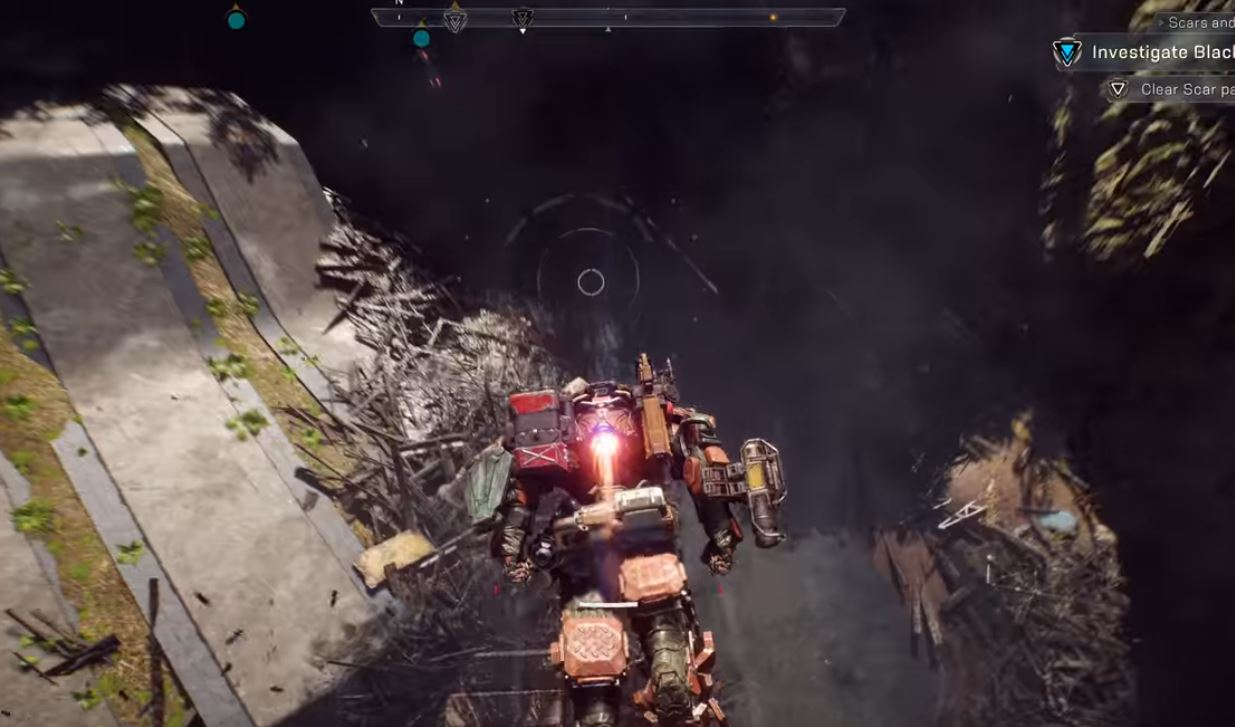
\includegraphics[width=\fullwidth]{assets/anthem-markers}
	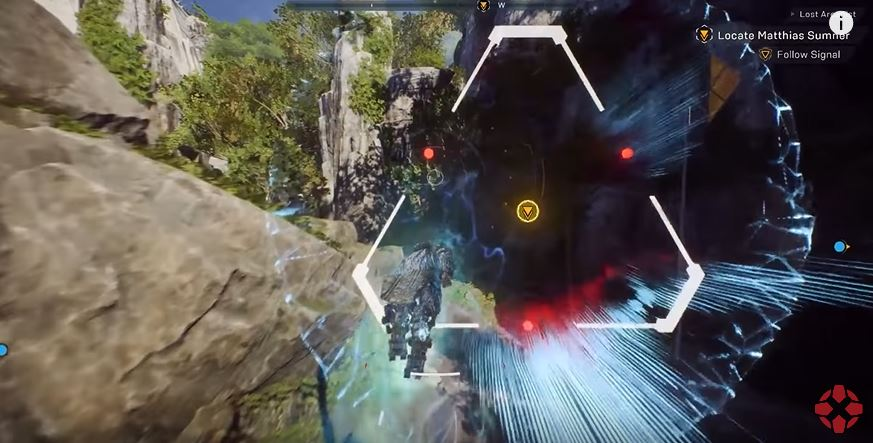
\includegraphics[width=\fullwidth]{assets/anthem-markers2}
	\caption{HUD UI markers from Anthem E3 Gameplay Demo\cite{anthem-e3}}
	\label{fig:anthem-hud-markers}
\end{figure}

One possible general use case is manage objects' lifetime based on culling\footnote{culling is hiding objects from rendering to improve performance} objects from rendering. Obviously since the player cannot see them when it's outside the view of the screen, we do not want to render them (shading, particles, textures) in order to improve performance. But re-creating the instances of world objects when player puts them into view again could be expensive, and cause stutter and lag when player looks around too fast. An object pool is applicable such that the objects that need to be rendered could be checked out, and returned when they no longer need to be rendered. See figure \ref{fig:culling} as an example for it used in Horizon Zero Dawn\cite{hzd}.\bs
\\

\iftwocolumns
\end{multicols}
\fi
\begin{figure}[H]
	\centering
	\begin{subfigure}[b]{0.49\textwidth}
		\centering
		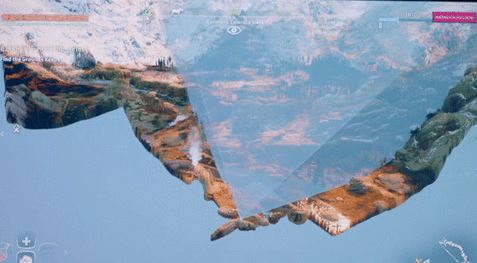
\includegraphics[width=\textwidth]{assets/culling-1}
	\end{subfigure}
	~
	\begin{subfigure}[b]{0.49\textwidth}
		\centering
		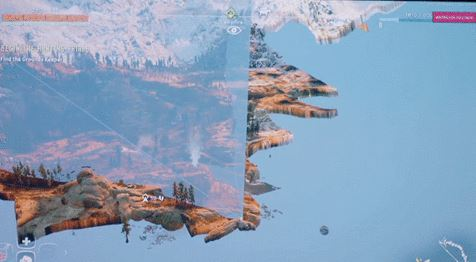
\includegraphics[width=\textwidth]{assets/culling-2}
	\end{subfigure}

	\caption{Culling of the world outside of player's field of view in the game Horizon Zero Dawn}
	\label{fig:culling}
\end{figure}
\iftwocolumns
\begin{multicols}{2}
\fi

\subsection{Prototype}

The \textit{prototype} design pattern helps when we need to create an object that is similar to an existing one, but instantiating a new instance is relatively expensive.\bs
\\
For instance, suppose we have a procedurally generated 3D model of a rock and we want to clone this model all over the place $N$ times.\bs
\\
We could just generate $N$ rocks like how we generated the first one using the same random seed.\footnote{Procedurally generation relies on pseudo-random or noise, which are based off of a seed.} The problem is for every clone of the rock, there are computational overheads that hinders efficiency: such as re-computing the normal vectors from all the faces of the polygon, or recalculating the UV coordinates for the texture.\bs
\\
Using the prototype design pattern, we implement a clone method to the rock object that copies all its data to a new instance, thereby avoiding the re-computation overheads.

\subsection{Singleton}\label{ssection:singleton}

The singleton pattern involves creating a single instance of a class and make sure that only one is created and used\cite{tp-singleton}. The singleton pattern provides a global accessor to the client such that it can be accessed everywhere. Thus, it is said singletons are glorified global variables.\cite{ood-singleton, sm-singleton}\bs
\\
In game development, singletons can be used for for system managers. i.e. a single manager class that overlooks and orchestrates UI system or a system to track achievements. 
% (see section \ref{ssection:ecs} for component-entity-system architecture where a single system manages multiple objects).\bs
\\
Singletons are also useful for configuration classes and shared resource accessing classes.\cite{ood-singleton} An example in game development is levels and personalization libraries (customization) where we load them into memory during loading screen initially. After-which their instance can be accessed via a static function call.\bs
\\
Typical singleton class implementation holds a static reference to itself and a static getter that returns that reference (figure \ref{fig:singleton}). In singleton implementations, concept of \textit{Lazy implementation}, where we do not initialize and allocate the memory for the object until client actually requests it.

\begin{figure}[H]
	\centering

	\scalebox{0.75}{
		\begin{tikzpicture}
			\begin{class}{Singleton}{0,0}
				\attribute{-instance: Singleton*}
				\operation{+Singleton():}
				\operation{+getInstance(): Singleton*}
			\end{class}
		\end{tikzpicture}
	}

	\caption{Generic singleton UML class diagram}
	\label{fig:singleton}
\end{figure}

An example of Singleton implementation for an simple achievement tracker in sample code in section \ref{code:singleton}.

% Two columns end
\iftwocolumns
\end{multicols}
\fi